\part{Descent and contradiction}
\section{Port graphs from cube exclusion}\label{sec:ports}

Network compression can bring many wires to a single vertex. To restore
bounded degree, Section~\ref{subsec:refresh} replaces all-pairs demands
among that vertex's ports by wires on a sparse graph. The metric estimate
this replacement requires is a Poincar\'e inequality, uniform over all
spectral placements of the ports. We show that the cube exclusion of
Section~\ref{sec:prices} gives graphs with precisely this property.

Let $G$ be a symmetric stochastic matrix on a finite vertex set $V$
and assign a point $x_i$ of a spectral space to each vertex $i$. The
mean squared length of a step of $G$ and the mean squared distance
between two independent uniform vertices are, respectively,
\[
 \mathcal E_G(x)=\frac1{|V|}\sum_{i,j\in V}G_{ij}d(x_i,x_j)^2,
 \qquad
 \mathcal V(x)=\frac1{|V|^2}\sum_{i,j\in V}d(x_i,x_j)^2.
\]

\begin{definition}\label{def:ports}
A field \emph{has ports} if it admits a family of regular, symmetric
multigraphs of unbounded order and bounded degree, and a constant
$\gamma$ such that
\[
 \mathcal V(x)\le\gamma\mathcal E_G(x)
\]
for every graph in the family and every assignment into a spectral space
over the field. Here $G$ denotes normalized adjacency. A diagonal arc
keeps the walk at its current vertex.
\end{definition}
This property depends only on the characteristic, since it concerns
only joint prices of binary wires (Lemma~\ref{lem:comparison}).
By Theorem~\ref{thm:geometry} one may test either finite spectral
points or complete $\operatorname{CAT}(0)$ spectral spaces. Testing
an assignment that is constant on each of two components and takes two
distinct values shows that every port graph is connected.

For use in Section~\ref{subsec:refresh}, we may take the graphs to be
loopless, of arbitrarily large power-of-two order and of one fixed
power-of-two degree. Given a graph of order $M$, duplicate enough
vertices to reach the next power of two. Keep the old edges between
the original representatives, join each duplicate to its representative,
and pad with holding arcs to a fixed power-of-two degree. To compare any
pair, follow the path through its two representatives. A uniform endpoint
chooses any particular representative with probability at most $2/M$.
The mean squared distance from a vertex to its representative is controlled
by a constant times the new edge energy, since each such pair is an edge
and the degree is bounded. The triangle inequality therefore gives a
uniform Poincar\'e bound after duplication. To remove loops, take two
copies of this graph. Replace each holding arc by a crossing to the
corresponding vertex in the other copy, and join every such pair of vertices
by as many additional parallel edges as the previous degree. The degree
doubles. The same comparison through representatives again gives a
uniform bound.

\begin{proposition}\label{lem:refresh-graph}\label{lem:ports}
If a finite field $F$ has a largest spectral flat dimension $k$, then
$F$ has ports.
\end{proposition}

\subsection{Construction of the port graphs}\label{app:refresh-graph}

The proof of Proposition~\ref{lem:refresh-graph} starts on a finite
Grassmannian. The quadrilateral inequality gives an upper bound on the
mean squared distance between complementary subspaces in terms of the
mean for adjacent ones. Equality would realize the excluded cube, so
there is a uniform gain. We use this gain twice. First, it yields sparse
matrices whose Poincar\'e constants grow more slowly than the exponent
governing their orders. Then a graph product turns this disparity into
a uniform bound at fixed degree.

The product uses the two equally weighted sets of transitions in the
balanced replacement product of Reingold, Vadhan and Wigderson
\cite[Definition~6.6]{RVW}. For the corresponding nonlinear spectral
comparison, see Mendel and Naor \cite[Theorem~1.13(V) and \S8]{MendelNaor}.
Their Ces\'aro estimates for the two-map nonlinear spectral gap in Hadamard
spaces appear in \cite[Corollary~1.9]{MendelNaorBarycentric}
and \cite[Theorem~3.4]{MendelNaorHadamard}. We give the one-map
lazy-walk estimate with the constants needed here.

Let $\mathcal X_F$ be the class of complete $\operatorname{CAT}(0)$
spectral spaces over $F$. By Theorem~\ref{thm:geometry}, every spectral
wire pseudometric embeds in a member of $\mathcal X_F$ after identifying
points at distance zero. Completeness permits us to take barycenters.
Write $\ell=k+1$ and let $Q_\ell=\{0,1\}^\ell$ be the excluded set of
cube corners with the Euclidean metric. Squared distances on $Q_\ell$
are Hamming distances. A matrix
$G$ has \emph{bound} $\gamma$ if $\mathcal V(x)\le\gamma\mathcal E_G(x)$
for every assignment into every member of $\mathcal X_F$. In a regular
graph we count both directions of an edge and count a loop as one diagonal
arc.

\subsubsection{A strict inequality on the Grassmannian}
Fix a power of two $m>\ell$, put
$W=\mathbb F_2^{2m}$, and let $\mathcal G$ consist of its $m$-dimensional
subspaces. The binary field here indexes the subspaces. Their images
lie in a spectral space over the coefficient field $F$, of arbitrary
characteristic. Given a map of $\mathcal G$ into $X$, let $B_r$ be the mean
squared distance over ordered pairs $(U,V)$ with $\dim(U+V)=m+r$.
Thus $B_1$ averages over adjacent subspaces, which meet in a hyperplane
of each, while $B_m$ averages over complementary subspaces.

\begin{lemma}\label{lem:wire-grassmann-gap}\label{lem:grassmann-gap}
There is an $\eta>0$, independent of $X\in\mathcal X_F$ and the map, such
that $B_m\le(m-\eta)B_1$.
\end{lemma}

\begin{proof}
By \eqref{eq:cur-quad}, the sum of the two squared diagonals of a
quadrilateral is at most the sum of the four squared sides. At
equality its opposite sides have equal lengths, as shown after
\eqref{eq:cur-quad}.

For $r,s>0$ with $r+s\le m$, take spaces $K,R_0,R_1,S_0,S_1$ in direct
sum of respective dimensions $m-r-s,r,r,s,s$. The four spaces
$K+R_i+S_j$ form a quadrilateral indexed by $i,j\in\{0,1\}$. Under a
uniform random automorphism of $W$, each ordered pair is uniform on all
pairs with its given sum dimension. Averaging the quadrilateral inequality
yields
\[
 B_{r+s}\le B_r+B_s,\qquad B_r\le rB_1.
\]
Suppose for a moment that $B_1=1$ and $B_m=m$. Then $B_r=r$ for every
$r$, by $B_m\le B_r+B_{m-r}$ for $0<r<m$. Every quadrilateral just used
is an equality configuration, since the deficits of all its translates are nonnegative
and have average zero.

Fix $0<r<m$ and independent columns $u_1,\ldots,u_r,w_1,\ldots,w_r$ in
$W$, with respective spans $U,U'$. Complete them by $m-r$ further
independent columns of span $S$. The image distance between $S+U$ and
$S+U'$ is independent of this choice of completion. Indeed, replacing one
completion column by a vector outside the current total span preserves the
distance by equality of opposite sides in the quadrilateral of type
$(r,1)$. These replacements connect all completions. To see this, for any
independent tuple of length less than $2m$ with a fixed prescribed
subtuple, one can simulate any independence-preserving change of a single
free column by these replacements. If the desired new column belongs to
the present span, first replace the old one by a vector outside the span.
This puts the desired column outside the new span. Arbitrary
independence-preserving changes connect the tuples by extending them to full
bases and using elementary column operations fixing the prescribed subtuple.
These are generated by additions on the remaining columns over
$\mathbb F_2$ (first modulo the prescribed subspace, then adding its
columns). Record only the changes to the original tuple.

The resulting common distance is also invariant when one of the $2r$
original columns $z$ is changed to a column $z'$ outside their span.
For this move choose the completion to contain $z+z'$ and extend it independently. The
total spans before and after this choice are the same, and neither
$S+U$ nor $S+U'$ changes. Since $2r<2m$, connectivity of the column
moves applies again. Every pair with sum dimension $m+r$ has such a
presentation, so every such squared distance equals $B_r=r$.

Choose $\ell$ disjoint pairs of columns and another $m-\ell$ columns,
all independent. The spaces spanned by the common columns and one choice
from each pair have squared image distances equal to the number of
differing choices, since $\ell<m$. Their images are an isometric copy
of $Q_\ell$.

Finally, if $B_1=0$ then $B_m=0$. If the asserted strict uniform gap
failed, we could rescale a sequence of configurations to have $B_1=1$
and $B_m\to m$. All entries of the finite distance arrays are bounded since
$B_r\le rB_1$ for every $r$. Take a convergent subsequence. Every array
is realizable up to scale over $F$, so the ultralimit procedure of Section~\ref{sec:limits}
realizes its limit up to scale as well. In a corresponding rescaled
geodesic completion this limiting map has $B_1=1$ and $B_m=m$. The
equality argument produces the excluded $Q_\ell$, a contradiction.
\end{proof}

\subsubsection{Sparse matrices on rapidly growing sets}
Decrease $\eta$ if necessary and choose $\varepsilon>0$ so that
$1<\alpha=(m-\eta)(1+\varepsilon)<m$. For every power of two $D\ge2$
and every integer $j\ge0$, we construct a symmetric stochastic matrix on
$D^{m^j}$ vertices with at most $C_jD$ entries in the support of each row
and with bound $C'\alpha^j$. Here $C_j$ may depend on $j$, whereas $C'$
is independent of both $j$ and $D$.

Start with the uniform matrix at size $D$. Given a matrix at size $N$,
let $E=\mathbb F_2^{\log_2 N}$ and take $\Omega=E^m$ as the new vertex
set. Fix an ordered basis in each $U\in\mathcal G$. A uniformly random
linear map $W\to E$ defines a uniform vertex of $\Omega$ at each $U$ by
reading its basis images. For a complementary pair of subspaces the two
vertices are independent. For an adjacent ordered pair $(U,V)$ of
subspaces they are independent conditional on the map on $U\cap V$, and
each conditional vertex is uniform in a fiber of size $N$. For each
endpoint these fibers partition $\Omega$, with uniform fiber weights.
Apply Lemma~\ref{lem:wire-grassmann-gap} to the points assigned to these
vertices and average over the random map. It bounds $\mathcal V$ by
$m-\eta$ times the average of the adjacent-pair expectations.

Fix one ordered adjacency $(U,V)$. For each value of the intersection
map, choose a bijection from the fiber at $U$ to the corresponding fiber
at $V$. Together these bijections give a permutation $\pi$ of $\Omega$.
On each fiber at $U$ place a copy of the preceding matrix, of bound
$\gamma$, and call their union $G_{UV}$. Let $P_\pi$ be the symmetric
average of the permutation matrix and its inverse. For the two conditional
vertices $a,b$, the vertex $\pi^{-1}(b)$ is uniform in the same fiber
as $a$ and independent of $a$ there. Comparing through $\pi^{-1}(b)$
and averaging over the fibers gives
\[
 \mathbb E\,d(x_a,x_b)^2\le
 (1+\varepsilon)\gamma\,\mathcal E_{G_{UV}}(x)
 +(1+1/\varepsilon)\mathcal E_{P_\pi}(x).
\]
The first term uses independent uniform vertices in a single fiber.
For the second, $b$ is uniform on $\Omega$, so the mean squared
distance from $x_{\pi^{-1}(b)}$ to $x_b$ is the permutation-edge energy.

Average the two weighted matrices over all ordered adjacencies and
normalize their sum to be stochastic. The Grassmannian estimate bounds
$\mathcal V$ by the energy of this matrix times
\[
 (m-\eta)\bigl((1+\varepsilon)\gamma+1+1/\varepsilon\bigr)
 =\alpha\gamma+(m-\eta)(1+1/\varepsilon).
\]
Since $\alpha>1$, iteration gives the bound $C'\alpha^j$. There are
only a fixed number of ordered adjacencies, depending on $m$, so each
step increases the support per row by at most a fixed multiple of the
old support plus a constant. At step $j$ the support is at most $C_jD$.

We realize each such matrix $G$ by a regular multigraph at a loss of
at most two in the bound. Choose a power of two $h$ with
$2C_jD\le h\le4C_jD$, increasing $C_j$ to at least one. Form symmetric
arc counts $\lceil h G_{uv}/2\rceil$ and pad each row to total $h$ with
loops. Before padding the row sum is at most $h/2+C_jD\le h$, and the new
energy is at least half the previous energy.

\subsubsection{Bounded-degree amplification}
The extension step replaces each vertex by a graph whose vertices
serve as ports. Within each copy the mean squared edge length controls
dispersion around the barycenter. Between copies a matching of ports realizes several steps of
the old walk. We first estimate the energy of these longer walks.

Let $G$ have bound $\gamma\ge1$,
put $A=(I+G)/2$, and, for even $t\ge2$, put $S=t^{-1}\sum_{h=1}^t A^h$.
Then $S$ has bound at most $C_0(1+\gamma/t)$ for a universal $C_0$.
To prove this, recall that a finite probability distribution on a complete
$\mathrm{CAT}(0)$ space has a barycenter minimizing the mean squared
distance. The midpoint inequality makes each minimizing sequence Cauchy, and
the geodesic squared-distance inequality with the interpolation fraction
tending to zero shows that the mean at $z$ exceeds the minimum by at
least the squared distance from $z$ to the barycenter.

Starting at $x_i^0=x_i$, let $x_i^{g+1}$ be the barycenter of the points
$x_j^g$ under row $i$ of $A$. Set
\[
 E_g=\frac1{|V|}\sum_{i,j}A_{ij}d(x_i^{g+1},x_j^g)^2,
 \qquad D_g=\frac1{|V|}\sum_i d(x_i^g,x_i^0)^2.
\]
Start a length-$h$ walk from the uniform law. Condition on the walk through its
penultimate vertex and apply the barycenter inequality with the initial
point as the test point. Repeat backwards through the walk. Stationarity
gives $\mathcal E_{A^h}(x)\ge D_h+\sum_{g<h}E_g$. Summing in $h$, using
$D_0=0$, yields a $0\le g<t/2$ with
\[
 D_g+(t/2)E_g\le2\mathcal E_S(x).
\]
Comparison through $x_i^{g+1}$ bounds $\mathcal E_G(x^g)\le4E_g$, since
half of row $i$ of $A$ comes from staying at $i$. Comparing $x_i^0,x_j^0$
through $x_i^g,x_j^g$ now gives
\[
 \mathcal V(x)\le 3(2D_g+\mathcal V(x^g))
 \le3(2D_g+4\gamma E_g)
 \le\max\{12,48\gamma/t\}\mathcal E_S(x).
\]

Fix $j$ large and then $D$ large, both specified below. As a graph on a
set of ports take the rounded graph $H$ just constructed on $Q=D^{m^j}$
vertices, with degree $h$ and bound $\beta=\max\{1,2C'\alpha^j\}$.
Put $b=2h$ and $t=m^j/4$, an even power of two for large $j$. We can
ensure $t(2b)^t\mid Q$ because all quantities are powers of two, $2b\le16C_jD$,
and for sufficiently large $D$,
$t(16C_jD)^t\le D^{4t}=Q$.

Given a symmetric $b$-regular graph with normalized matrix $G$, replace
each vertex by a cloud of $Q$ ports. On the new vertex set use $H$ inside
each cloud with probability $1/2$ and otherwise use a port
involution realizing the transitions $S$ between clouds for uniform
ports. Each $A^i$ has denominator dividing $(2b)^t$, so $QS$ is integral.
At cloud $u$ partition the ports into sets of sizes $QS_{uv}$. Pair the parts indexed by $u,v$ and by $v,u$,
using fixed points for self-transitions. Taking the $h$ arcs of $H$ and
$h$ copies of the matching arc at each port gives degree $b$ again.

Let $y_u$ be the barycenter of cloud $u$ and let $V_0$ be the mean squared
distance to one's own barycenter. Write $E_{\rm in},E_{\rm match}$ for the
mean internal and matching energies. By minimization and the bound on $H$,
$V_0\le\beta E_{\rm in}$. The three-segment estimates via a matched pair
and via the two barycenters, respectively, give
\[
 \mathcal E_S(y)\le3(2V_0+E_{\rm match}),\qquad
 \mathcal V(x)\le3(2V_0+\mathcal V(y)).
\]
Since the new energy is $(E_{\rm in}+E_{\rm match})/2$, a new bound is
$C_1\beta(1+C_0(1+\gamma/t))$ with universal $C_1$, whenever the old bound
is $\gamma\ge1$. The coefficient $C_1 C_0\beta/t$ is
$O((\alpha/m)^j)$, so choose $j$ to make it less than $1/2$ and then
choose $D$ as above. Starting with a single vertex with $b$ loops, the
iteration gives graphs on the powers of $Q$, with a uniformly bounded
Poincar\'e constant and degree $b$.

The resulting family has unbounded order, fixed degree and a common
bound for every target in $\mathcal X_F$. This proves
Proposition~\ref{lem:refresh-graph}.



\section{Fixed wire identities from metric inequalities}
\label{sec:motifs}

A product of wires can be replaced by a sum of products on a different
graph. For compression, we need a bound on the total wire width in
every summand after its endpoints are regrouped. Theorem~\ref{thm:conversion} turns a comparison
of squared wire distances into a bound on the widths in each summand.
Lemma~\ref{lem:motif} supplies this comparison for a six-party graph
that admits two ways of regrouping its endpoints. Both results hold
over an arbitrary field, denoted here and in Section~\ref{sec:compressor}
by $\mathbb F$.

Fix a finite set of at least two parties, a multiset $D$ of demand edges,
and a connected spanning multigraph $S$ of supply edges. Each edge has distinct endpoints.
For nonnegative integer widths $b=(b_e)_{e\in D}$,
let $W_D(b)$ be the product of identity tensors of dimensions $2^{b_e}$
on their respective edges. Define $W_S(c)$ similarly. Give the edges
positive rational masses $p_e$ on $D$ and $q_e$ on $S$, and set
\[
  \|b\|_p^2=\sum_{e\in D}\frac{b_e^2}{p_e},\qquad
  \|c\|_q^2=\sum_{e\in S}\frac{c_e^2}{q_e}.
\]
For a spectral point $F$ on these parties over $\mathbb F$, write $d_e$ for its
wire distance on the endpoints of $e$. In particular,
$\log_2 F(W_D(b))=\sum_{e\in D}b_e d_e$.
We use this comparison on six parties to shrink the total width and later on a block of ports to restore bounded degree.
The squared-distance energies in Equation~\eqref{eq:motif-rayleigh} are dual to the width energies above. For
example, the maximum of $\sum_{e\in D}b_e d_e$ over real $b\ge0$ with
$\|b\|_p\le1$ is $(\sum_{e\in D}p_e d_e^2)^{1/2}$.
The next theorem turns this comparison into exact identities for
integer widths.

\begin{theorem}[Conversion of a fixed motif]
\label{thm:conversion}
Let $H\ge0$ and suppose that for every such spectral point,
\begin{equation}
 \sum_{e\in D}p_e d_e^2\ \le\ H\sum_{e\in S}q_e d_e^2 .
 \label{eq:motif-rayleigh}
\end{equation}
For every $H'>H$ and all $b$, there is an ordinary sum identity
\begin{equation}
 W_D(b)=\sum_\alpha
       \left(\bigotimes_v L_{v,\alpha}\right) W_S(c_\alpha),
 \qquad
 \|c_\alpha\|_q^2\le H'\|b\|_p^2+O(1).
 \label{eq:motif-conversion}
\end{equation}
The constant in the energy estimate is independent of $b$. The identities
use finitely many scalar parameters $\kappa$ subject to fixed integer
polynomial equations with a solution in $\mathbb F$. They hold over every
commutative unital ring with any assignment satisfying these equations.

With $M=\max(\{0\}\cup\{b_e:e\in D\})$, each index $\alpha$ consists of
a fixed number of integers of magnitude $O(M+1)$. Admission and supply
widths are computable in $\operatorname{poly}(\log(2+M))$ bit operations.
Given the index and its incident bit strings, an entry of $L_{v,\alpha}$
is specified as zero or as a monomial in $\kappa$ of degree $O(M+1)$.
Its description is computable in time polynomial in $M+2$ with an
absolute exponent.
\end{theorem}

\begin{proof}
Choose a rational $R$ strictly between $\sqrt H$ and $\sqrt{H'}$.
The case $b=0$ uses one unit term. Otherwise round $b/\|b\|_p$
coordinatewise upwards to a sufficiently fine fixed rational grid. This
gives one of finitely many vectors $z$ with $\|z\|_p\le 1+\epsilon$,
where $(1+\epsilon)\sqrt H<R$. Weighted Cauchy--Schwarz and
Equation~\eqref{eq:motif-rayleigh} give
\[
  \sum_{e\in D}z_e d_e
   <R\left(\sum_{e\in S}q_e d_e^2\right)^{1/2}
    =\max_{w\ge0,\,\|w\|_q\le R}\sum_{e\in S}w_e d_e .
\]
Indeed the supply norm on the right is positive. If it vanished, a
product of binary wires along a spanning tree would have value one,
whereas it restricts to the two-copy diagonal, of value two. Rational
approximation inside the supply ball and compactness of the spectrum
give a finite list $\mathcal W$ of nonnegative rational $w$ that suffices
for the strict inequality for every $z$ and $F$.

Choose a large common denominator multiple $B$ for both grids. For each
$z$, every spectral point strictly orders $W_D(Bz)$ below
$Y=\bigoplus_{w\in\mathcal W}W_S(Bw)$. By strict spectral comparison
(Lemma~\ref{lem:spectral-comparison}), some fixed $K_z$ copies of $Y^{\otimes h}$
restrict to $W_D(hBz)$ for every $h\ge1$. Expand these direct sums into
an ordinary sum of images of supply tensors under local maps. Each
base term has supply-width vector of norm at most $hBR$ by the triangle
inequality. Its index fits in
\[
   s=\left\lceil\log_2(\max_z K_z)+h\log_2|\mathcal W|\right\rceil
\]
bits. We may make $s/(hB)$ as small as desired by choosing $B$ large
first and then $h$ large. Fix $B,h$ at these values. Introduce one
parameter for each entry of each base local map, with the base
identities themselves imposed entrywise as polynomial equations.
These finitely many equations have integer coefficients and a simultaneous
solution in $\mathbb F$.

For the given nonzero $b$, take $u=\lceil\|b\|_p/(hB)\rceil$ copies of
the base identity at $z$. Its demand widths $uhBz$ dominate $b$. Fix
all surplus demand bits to zero at both ends. To avoid listing a separate
outer term for every sequence of $u$ base selectors, group sequences
by their total supply payload $v=(v_e)_{e\in S}$. Allow every integral
$v\ge0$ with $\|v\|_q\le uhBR$, including values that come from no
sequence. For this one outer index, use width $c_e=v_e+us$ on supply
edge $e$.

At each party, read the $us$ selector bits on every incident supply edge.
Require the lists to agree, require every selector to be valid, and
require the sequence's total payload vector to be the stated $v$.
Use the selectors in order to split each incident payload into the
corresponding base fields. Return the product of the selected base-map
entries, with the demand padding prescribed above. Failure of any check
gives a zero entry. Since the supply graph is connected, a surviving
assignment of selector copies is determined by a single global sequence.
Conversely every sequence gives exactly one such assignment. Summing
the payload bits therefore reproduces the product identity, with each
sequence counted once in its $v$-term. This proves the identity over every
ring satisfying the base equations.

Writing $\mathbf 1$ for the all-ones vector on $S$, the resulting widths
satisfy
\[
  \|c\|_q\le uhB\left(R+\frac{s}{hB}\|\mathbf 1\|_q\right).
\]
Take the selector fraction small enough that the factor in parentheses
is strictly less than $\sqrt{H'}$. Since $uhB\le\|b\|_p+hB$, squaring
gives the bound in Equation~\eqref{eq:motif-conversion} because the strict gap in the
quadratic coefficient absorbs the linear term up to a constant.

The outer index $v$ has a fixed number of coordinates of size $O(M+1)$.
Deciding the grid cell of $b/\|b\|_p$, computing $u$, and testing its
norm bound use integer comparisons after clearing fixed denominators and
squaring nonnegative quantities. All operands have $O(\log(2+M))$ bits.
To evaluate one map entry, scan the $u=O(M+1)$ fixed-size selectors and
their fields, incrementing one parameter exponent per copy. All local
dimensions of the base identities are constants. Even rescanning all
incident strings to locate each successive field takes only
$O((M+2)^2\operatorname{polylog}(M+2))$ bit operations with a fixed
multiplicative constant. This gives the stated uniform exponent.
\end{proof}

\subsection{Two layouts on six parties}
The endpoints $A,B$ represent sites where several vertices have been
packed together. We pair their demand wire $AB$ with a second demand
wire $CD$. The placement of $D$ may already be fixed by another
occurrence of the motif. We retain the freedom to place $C$ at either
$A$ or $B$, and use two auxiliary parties $M,N$ to make a different
group of supply wires local in each case. For a related packing
construction, see \cite[Appendix~D]{falseeth}.

Consider the six-party graph with demands $AB,CD$ and supply
groups
\[
 G_1=\{AC,AM,CM,DN\},\qquad G_2=\{BC,BN,CN,DM\}.
\]
Under the first layout, identify the parties within $ACM$ and within
$DN$. Under the second layout, identify the parties within $BCN$ and
within $DM$. The two demand wires remain part of the local maps. In each
layout every supply wire in the corresponding group can be summed at a
single position, as indicated in Figure~\ref{fig:motif-layout}.

\begin{figure}[!htbp]
\centering
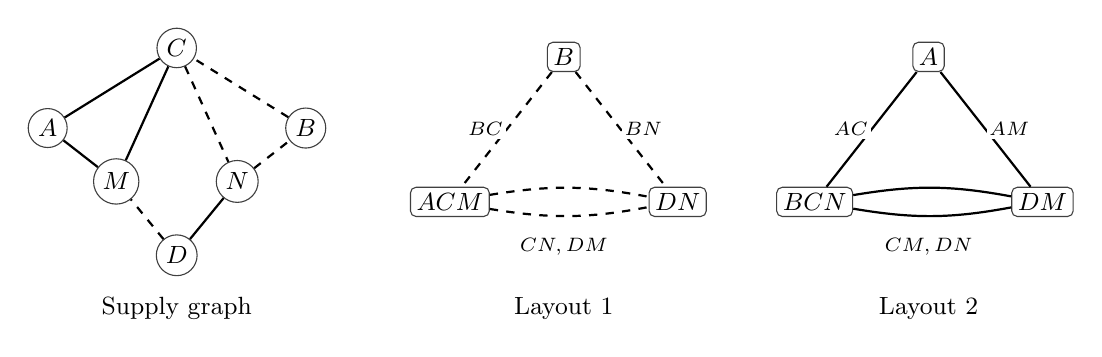
\begin{tikzpicture}[scale=1.13,
 pt/.style={circle,draw=black!75,fill=white,inner sep=1.7pt,font=\small},
 grp/.style={draw=black!75,fill=white,rounded corners=2pt,
              inner sep=2.2pt,font=\small},
 tag/.style={font=\scriptsize,fill=white,inner sep=1pt}]
 \begin{scope}
 \node[pt] (a) at (-1.45,.15) {$A$};
 \node[pt] (b) at (1.45,.15) {$B$};
 \node[pt] (c) at (0,1.05) {$C$};
 \node[pt] (m) at (-.68,-.45) {$M$};
 \node[pt] (n) at (.68,-.45) {$N$};
 \node[pt] (d) at (0,-1.28) {$D$};
 \draw[thick] (a)--(c)--(m)--(a) (d)--(n);
 \draw[thick,dashed] (b)--(c)--(n)--(b) (d)--(m);
 \node at (0,-1.88) {\small Supply graph};
 \end{scope}
 \begin{scope}[xshift=4.35cm]
 \node[grp] (t) at (0,.95) {$B$};
 \node[grp] (l) at (-1.28,-.68) {$ACM$};
 \node[grp] (r) at (1.28,-.68) {$DN$};
 \draw[thick,dashed] (t)--node[tag,left] {$BC$} (l)
                  (t)--node[tag,right] {$BN$} (r)
                  (l) to[bend left=10] (r)
                  (l) to[bend right=10] (r);
 \node[tag] at (0,-1.18) {$CN,DM$};
 \node at (0,-1.88) {\small Layout 1};
 \end{scope}
 \begin{scope}[xshift=8.45cm]
 \node[grp] (t) at (0,.95) {$A$};
 \node[grp] (l) at (-1.28,-.68) {$BCN$};
 \node[grp] (r) at (1.28,-.68) {$DM$};
 \draw[thick] (t)--node[tag,left] {$AC$} (l)
           (t)--node[tag,right] {$AM$} (r)
           (l) to[bend left=10] (r)
           (l) to[bend right=10] (r);
 \node[tag] at (0,-1.18) {$CM,DN$};
 \node at (0,-1.88) {\small Layout 2};
 \end{scope}
\end{tikzpicture}
\caption{Two placements of the supply graph for the demands $AB$ and $CD$.
Layout 1 contracts
the solid edges $G_1$ and retains the dashed edges $G_2$. Layout 2 contracts $G_2$ and retains $G_1$. The two parallel edges
in each layout represent distinct supply wires.}
\label{fig:motif-layout}
\end{figure}

\begin{lemma}[Six-party energy saving]
\label{lem:motif}
Take $t=1/2$ and give $AB$ and $CD$ masses
$r=t^2/(1-t^2)=1/3$ and $1$, respectively. There are rational positive
supply masses, of total $1+r$ in each group, for which
\begin{equation}
 r d_{AB}^2+d_{CD}^2\ \le\ \frac{31}{16}\sum_{e\in G_1\cup G_2}q_e d_e^2
 \label{eq:motif-six}
\end{equation}
holds for every six-point configuration in a $\mathrm{CAT}(0)$ space,
and hence for every assignment in a spectral wire pseudometric over $\mathbb F$.
\end{lemma}

\begin{proof}
Embed the wire distances into a $\operatorname{CAT}(0)$ space by Corollary~\ref{cor:spectral-geodesic} and Lemma~\ref{lem:catzero}. Write $XY$ for the distance between $X$ and $Y$. Give the pairs $(AC,BC)$, $(AM,BN)$, $(CM,CN)$ and $(DM,DN)$ effective coefficients $1/2,1/4,5/6,1$, respectively. Let $E$ be their weighted sum of squared lengths. Put $U=[C,M]_{1/3}$ and $V=[C,N]_{1/3}$. Equation~\eqref{eq:cur-cn} gives
\[
  \tfrac12 AC^2+\tfrac14 AM^2\ge\tfrac34 AU^2+\tfrac16 CM^2
\]
and the corresponding bound with $B,N,V$. Adding the remaining terms leaves $CM^2+CN^2+DM^2+DN^2$ in addition to $\tfrac34(AU^2+BV^2)$. At the midpoint $O$ of $MN$, the midpoint inequality bounds those four squares below by $2CO^2+2DO^2+MN^2\ge CD^2+MN^2$. Hence
\[
 E\ge\tfrac34(AU^2+BV^2)+CD^2+MN^2 .
\]
Convexity along geodesics gives $UV\le MN/3$, so $AB\le AU+BV+MN/3$. Weighted Cauchy--Schwarz gives
\[
 \tfrac13 AB^2\le\tfrac{25}{27}\bigl(\tfrac34(AU^2+BV^2)+MN^2\bigr).
\]
Thus $E$ bounds $\tfrac13 AB^2+CD^2$ from above. The effective coefficients sum to $31/12$ in each layout group. Dividing them by $31/16$ gives the required rational masses, of total $4/3$ per group.
\end{proof}

In the packing used in Section~\ref{sec:compressor}, a bit at each
endpoint marks it thick or thin. A fraction
$t^2=1/4$ of wires have two thick endpoints, and the packing distributes
their total mass over the remaining fraction $3/4$. This fixes $r=1/3$.
Fix any $31/16<H'<2$ in Theorem~\ref{thm:conversion} for this motif.
After choosing one term at each occurrence in a collection of motifs,
one common layout suffices to discard at least half of their total
supply energy. Indeed the surviving costs under the two layouts sum to
the entire supply energy. Before rounding widths to regularize the
degrees, the leading coefficient on the demand energy is therefore
$H'/2<1$. The construction in Section~\ref{sec:compressor} realizes both identifications consistently
when different occurrences share positions and preserves the strict
saving through rounding.
\section{Compression of a wire network}\label{sec:compressor}

Theorem~\ref{thm:compressor} gives an exact expansion of a wire network.
After $T$ blocks, the sum of the surviving widths in each term is
bounded by $2^{-T}$ times a quantity determined by the initial network.
A block has two stages. Several applications of the six-party identity
reduce the leading coefficient of a quadratic energy bound while
increasing the degree. The port graph then restores the original degree
with a multiplicative loss independent of the intermediate degree.
This independence permits iteration.

\subsection{Wire networks and local identities}

Let the base be a finite indexed directed multigraph with distinct endpoints
on every arc and with $d$ incoming and $d$ outgoing arcs at every vertex,
where $d$ is a power of two. Number the slots at each vertex separately in
each direction. Give each base arc $e:x\to y$ a displacement $\tau_e$ in a
binary vector space of lanes. The positions are the pairs $(x,g)$ of base
vertex and lane. The actual arcs over $e$ are
\[
       (x,g)\longrightarrow (y,g+\tau_e).
\]
Directions and slots index the wires. An actual arc of width $b_e$ equates
two strings of $b_e$ bits. The integer width, possibly zero, can vary from one
lane to another. With $P$ positions there are $Pd$ actual arcs. Give each
mass $p=1/(Pd)$ and put
\[
   \mathcal L=\sum_{e\,\text{actual}} b_e^2/p,
   \qquad \sum_{e\,\text{actual}} b_e\le\sqrt{\mathcal L}.
\]
To bound the energy of a concatenated wire, let $p_i$ and $b_i$ be
the masses and widths of its constituents. Cauchy--Schwarz gives
\[
        \frac{(\sum_i b_i)^2}{\sum_i p_i}\le\sum_i b_i^2/p_i.
\]
Thus a concatenated wire can inherit the total mass of its constituents
without increasing energy. Splitting it across integral slots incurs only
the rounding error estimated below.

Write $a_u$ for the string of incident half-wire indices at position $u$,
and $W((a_u)_u)$ for the product of the wire equalities. A substep gives an
identity of the form
\begin{equation}\label{eq:kernel}
 W((a_u)_u)=\sum_{\iota}\ \sum_{z}
   \prod_{v} K_{v,\iota}
       \big((a_u)_{\pi_\iota(u)=v},\,z|_v\big).
\end{equation}
Here $\iota$ is a list of admitted motif terms. The new topology, widths,
placement $\pi_\iota$ of old positions, and kernels are determined by this
list. The variable $z$ chooses one string per new actual arc, used at both
ends. A kernel consists of local ties, sums over local indices, and entries
of the maps in Theorem~\ref{thm:conversion}. After multiplying by arbitrary old
vertex factors and summing the $a_u$, every whole old factor belongs to the new
vertex $\pi_\iota(u)$. In this sum the two old half-wire indices can be
chosen separately, as their former equality has been expanded. Any uncontracted
indices of an old factor move with it. All identities below hold in every
commutative unital ring satisfying the fixed equations on the map entries.

\begin{theorem}[Iterated compression]\label{thm:compressor}
Suppose there are ports over $\mathbb F$ in the sense of
Definition~\ref{def:ports}. Use the family of connected loop-free symmetric regular
graphs of fixed degree and arbitrarily large power-of-two orders from
Section~\ref{sec:ports}. Its squared-distance Poincar\'e bound holds
with one constant for every spectral wire pseudometric over $\mathbb F$.
There exist a
power-of-two degree $d_0$, a positive integer $b_0$, a constant $C_2\ge2$
and finitely many motif templates, all fixed, with the following property.
Let a network of the stated form have $P_0$ positions of degree $d_0$,
maximum width $W_0$, and at least $Tb_0$ lane coordinates, for $T\ge1$.
It has an exact expansion by $T$ blocks of local identities
\eqref{eq:kernel}, ending at degree $d_0$. The same finite system of
parameter equations, satisfiable in $\mathbb F$, suffices for every network and $T$.
For every sequence of admitted terms,
\begin{equation}\label{eq:compress-bound}
  \sum_{e\,\mathrm{final}} b_e\le\sqrt{\mathcal L_T}
  \le 2^{-T}\big(\sqrt{\mathcal L_0}+O(P_0)\big).
\end{equation}
All intermediate wire and kernel fields have length at most
$C_2^T(W_0+1)$. At each final position, the recursive expansion of its
vertex tensor uses at most $C_2^T$ occurrences of vertices, map entries
and fields. This counts each initial factor and each map entry as an
unevaluated operation in the local contraction, with one occurrence
shared by all values of its hidden indices. For fixed arguments, a nonzero map entry contributes
a monomial of parameter degree at most $C_2^T(W_0+1)$.
\end{theorem}

\subsection{Packing the wire slots}\label{sec:compressor-slots}

The lane coordinates let us replicate each base arc in four endpoint
configurations. We mark each endpoint thick or thin. Thick positions
will merge at a fixed site, whereas thin positions can move to either
end of an assigned bundle. The assignment must move every occurrence
of a given old position together, even when several motifs meet there.

\begin{lemma}[Packing and placement of the wire slots]\label{lem:compressor-slots}
For every power-of-two base degree $d$, set $K=2^{2d+1}d$ and $Q=3K/4$.
There is a packing of the wire slots, using a number of lane coordinates
depending only on $d$, with the following properties. The two layouts
refer to the six-party motif of Figure~\ref{fig:motif-layout}.
\begin{enumerate}
\item Packing the thick positions produces $P/K$ new positions. Each
thick--thick bundle contains $K/4$ wires. Every other wire is assigned as
a $CD$ demand to the bundle of its thin $C$ endpoint, with $Q$ per bundle.
\item In either layout the packed endpoints $A,B$ and the image $D^*=\pi(D)$
of the other endpoint have distinct bases in each motif. Each of these three
roles occurs exactly $dQ$ times per new position.
\item Translation of the remaining lane preserves the assignments, placements
and unweighted slots. Slot numbering, including the padding
to any admissible output degree, can be determined by bounded-size lists
per new position after a greedy scan of the base.
\end{enumerate}
\end{lemma}

\begin{proof}
Color the base greedily with $2d+1$ colors. Split the lane as $(U,h,j,g)$,
where $U$ supplies one bit per color, $h$ indexes the $d$ outgoing slots,
$j$ is a tag in a binary vector space of order $J$, and $g$ is the remaining
lane. We determine $J$ below. Call a position thick if its base-color bit
is $1$, and thin otherwise. Put $K=2^{2d+1}d$, the number of pairs $(U,h)$.
Along a base arc the endpoint colors are distinct. With $j,g$ fixed at one
end, the two tests use distinct free bits of $U$ up to translations. They
are independent fair tests, also independently of $h$ at either end.
Consequently each of the four endpoint types occurs $K/4$ times.

For given $x,j,g$ pack all thick positions there into a single new one, with
base $(x,j)$ and lane $g$. There are $P'=P/K$ new positions. Bundle the
$K/4$ thick--thick wires of each base arc for fixed $j,g$ at its source by
concatenating them in a common order at both endpoints. The bundle runs from
a packed position $A$ to a packed position $B$. For every wire outside these
bundles take a thin end for $C$ and the other end for $D$. For thin--thin
wires take their old direction $C\to D$.

Give each base vertex $x$ an offset $\phi_x$. Assign each thin position
$(x,U,h,j,g)$ to the bundle with source $(x,j+\phi_x,g)$ on the outgoing
base arc of slot $h$. Every wire on which this position plays $C$ is assigned
to that bundle. To count these wires, fix the base, tag, remaining lane and
slot of its possible thin sources. The $d$ originally outgoing incidences
contribute $d(K/(2d))=K/2$ wires. The $d$ originally incoming incidences
from thick positions contribute $d(K/(4d))=K/4$. Thus each bundle receives
$Q=3K/4$ wires of type $CD$.

We choose the tag offsets so that $A,B,D^*$ always have distinct new bases.
The old base components of $A,B$ differ. For $C$ at old base $x$ with tag
$j$, and $D$ at $y$ on their old base arc $e$ in either direction, write
\[
          L_x=\{0\}\cup\{\tau_f^{\mathrm{tag}}: f\text{ leaves }x\}.
\]
The new tags of $A,B$ lie in $j+\phi_x+L_x$. A thick $D$ has tag
$j+\tau_e^{\mathrm{tag}}$, and the possible tags of a thin $D^*$ belong to
$j+\tau_e^{\mathrm{tag}}+\phi_y+L_y$. It suffices to impose, at each
incidence,
\[
      \phi_x\notin\tau_e^{\mathrm{tag}}+L_x,
      \qquad \phi_x+\phi_y\notin\tau_e^{\mathrm{tag}}+L_x+L_y.
\]
Greedy choice in base order works for any power of two
$J>2d((d+1)+(d+1)^2)$, since at most this many values are forbidden by
the first conditions and the already assigned neighbors in the second.

\smallskip
At every new position $d$ bundles start and $d$ bundles end, so each of
the roles $A,B$ occurs $dQ$ times. The thick $D$ endpoints at this position
contribute $2dK/4=dK/2$ occurrences of $D^*$, counting mixed arcs in both
old directions. The others are destinations of thin--thin arcs. Before
placement, for fixed base, tag and remaining lane, these contribute $dK/4$
occurrences, equally distributed over destination slot labels $h$. In
layout~1 the tag offset permutes the tags. In layout~2 each position receives
through $d$ incoming base arcs, each with a uniquely determined source tag
and remaining lane, and each carrying $K/4$ such occurrences from its
assigned slot. In both cases the total number of $D^*$ roles is
$dK/2+dK/4=dQ$.

Packing, bundle assignment, and the two choices of image depend on the
remaining lane only through the given arc translations. The common choice
of layout therefore preserves this symmetry. For each surviving occurrence,
label its parallel slots by the original $CD$ arc identifying the motif, the
surviving type, and the subdivision index. When a common deficit remains
after the degree calculation in Subsection~\ref{subsec:shrink}, add zero-width
arcs to the next tag cyclically at the same old base and remaining lane.
Number incoming and outgoing slots separately by sorting their identifiers,
expressing all remaining lanes relative to the vertex being numbered. The
orders transport from lane zero to every lane. Widths and term-dependent map
entries need never enter these identifiers.

Greedy coloring and tag selection each use a single scan of the indexed
base and bounded neighbor lists. After these scans the assignments can be
formed by listing the actual arcs by bundle, and the regularized slots by
their endpoints. The list sizes depend only on the fixed degrees and lane
coordinates consumed in this step. The sorted identifiers give the two
corresponding slot numbers and their displacement, as required for the
next level of the construction.
\end{proof}


\subsection{The energy estimate for one shrinking step}\label{subsec:shrink}

Use the masses of Lemma~\ref{lem:motif}. Write $t=1/2$, $r=1/3$, give the
two demands $AB,CD$ relative masses $r,1$, and give each supply type $e$ its
positive rational relative mass $q_e$. Each of the two supply groups has
total relative mass $1+r$. Fix $31/16<H'<2$ in Theorem~\ref{thm:conversion},
using the metric inequality of Lemma~\ref{lem:motif}, and choose $0<\delta_0<1$ such that
\[
                  \rho=\frac{H'}{2(1-\delta_0)}<1.
\]
With current degree $d$, the step works for every sufficiently large
power of two $d'$ as its output degree. For every term its energy satisfies
\begin{equation}\label{eq:compress-shrink}
        \mathcal L_{\mathrm{new}}\le \rho\mathcal L+O_{d,d'}(P^2).
\end{equation}
The fixed field and motif data may enter all implicit constants.

\paragraph{Packing and assignment.}
Apply Lemma~\ref{lem:compressor-slots}. There are $P'=P/K$ new
positions, with $K=2^{2d+1}d$. Each bundle concatenates $K/4$ thick--thick
wires between the packed endpoints $A,B$. Divide this payload into
$Q=3K/4$ integral pieces as evenly as possible and pair each piece
with one of the $Q$ demands $CD$ assigned to the bundle.

Give these two demands actual masses $rp,p$. Since $rQ=K/4$, the pieces
collectively inherit the mass of the bundled wires. A bundle of total width $b$
would cost $b^2/(Qrp)=b^2/((K/4)p)$ under perfectly equal division. By
Cauchy--Schwarz this is at most the original energy of its thick--thick
wires. Dividing an integer $b$ evenly into $q$ integers raises their sum of
squares above $b^2/q$ by at most $q/4$: their deviations are centered and
the variance of the two consecutive values is at most $1/4$.
Thus rounding costs at most $Q/(4rp)$ per bundle. There are $P'd$ bundles,
and each $CD$ wire keeps its energy. The total demand energy is therefore
at most $\mathcal L+O_d(P^2)$. Apply the wire identity of
Theorem~\ref{thm:conversion} with the masses of Lemma~\ref{lem:motif} to
each motif. After scaling masses by $p$, its additive cost is $O(1/p)$ per motif,
and there are $P'dQ=O_d(P)$ motifs. In every list of terms the total supply
energy is at most $H'\mathcal L+O_d(P^2)$.

\paragraph{Choosing the placement.}
The two layouts send each thin position to opposite ends of its bundle.
Because Equation~\eqref{eq:motif-conversion} is an identity before any
sites are identified, we can select a common layout after choosing the
motif terms.

The first supply group $G_1$ consists of the triangle on $A,C,M$ and the
edge $DN$. The second, $G_2$, consists of the triangle on $B,C,N$ and the
edge $DM$. Choose a single layout for the entire list of terms, retaining the
group of smaller total energy, with deterministic tie breaking. Each layout
first defines the placement $\pi$ of whole old positions. A thick position
goes to its packed site. A thin position goes to the $A$ of its assigned
bundle in layout~1 and to its $B$ in layout~2. This places every $C$ as
required. In every motif the $D$ map goes to $D^*=\pi(D)$, even if that old
position plays $C$ or $D$ elsewhere. Its old vertex factor thus moves only
once.

In layout~1 put the fresh $M$ at $A$ and the fresh $N$ at $D^*$. All edges
of $G_1$ become local. Of the surviving edges, $BC$ joins $B,A$, $BN$ joins
$B,D^*$, and $CN,DM$ join $A,D^*$. Layout~2 interchanges $A,B$ and $M,N$,
making $G_2$ local. The choice retains at most half of the total supply energy.

\paragraph{Regularizing the degree.}
Lemma~\ref{lem:compressor-slots} arranges that $A,B,D^*$ have distinct
bases in each motif and that each of these three roles occurs exactly $dQ$
times at every new position, in either layout.
The new arc mass is $p'=1/(P'd')=pKd/d'$. For every surviving type $e$ use
$m_e=\lfloor p q_e/p'\rfloor$ parallel arcs per occurrence, oriented by its
two roles in a fixed order. Take $d'$ large enough that $m_e>0$ and
$m_e p'\ge(1-\delta_0)p q_e$ for all types. Since each role occurs $dQ$
times, both the in-count and the out-count at every position are
\[
       dQ\sum_{e\,\text{surviving type}}m_e
       \le dQp(1+r)/p'=d'.
\]
Fill the common deficit with zero-width arcs as in
Lemma~\ref{lem:compressor-slots}. The slots commute with translations of the
remaining lane, so the new graph again has fixed displacements on its base
arcs. This symmetry concerns only the unweighted slots. Widths and map
entries may differ on every lane.

Split the surviving payload of width $b$ as evenly as possible among its
$m_e$ slots. The new cost is at most $b^2/(m_ep')+m_e/(4p')$.
The multiplicative loss relative to its supply energy is at most
$1/(1-\delta_0)$. For these fixed degrees there are $O_d(P)$ occurrences,
$m_e$ is bounded, and $1/p'=O_{d,d'}(P)$. Summing this estimate after the
choice of layout proves \eqref{eq:compress-shrink}.

\paragraph{Exact contraction and size of a kernel.}
Concatenating the thick--thick fields and slicing them identically at both
ends rewrites the old wire tensor as the product of the joint $AB,CD$
demands. Expand each with its selected motif identity, summing over lists
of selections. Put the maps for $C,D$ at the images of these old endpoints
and place all other maps by the selected layout. Every absorbed wire is
summed once inside its new position. The remaining wire bits are exactly the
bits allocated to parallel slots. This proves \eqref{eq:kernel}, including
when the layout depends on the term list. A new vertex receives boundedly many
old positions, since the number of slots and consumed coordinates is fixed.
It contains boundedly many maps and wire fields, by the role counts. If the
largest old width is $W$, each new or local field has length $O_{d,d'}(W+1)$,
by the bundle bound and Theorem~\ref{thm:conversion}. Concatenations and
slices are described by bounded lists of field identifiers, offsets and
lengths, even where two slice boundaries differ. Each map needs only the
compact term description and widths from the conversion theorem.
\subsection{Restoring the degree}\label{subsec:refresh}
Let $d_H$ and $\gamma_H$ be the degree and Poincar\'e constant of the
loop-free port graphs constructed in Section~\ref{sec:ports}.

Fix a power of two $d_0\ge \max\{4,d_H+1\}$.
Choose the last shrinking step so that its output degree $D$ is an order in the port family. Use the graph of that order on the $D$ ports. We give a step that
keeps all $P$ positions and returns their in- and out-degrees to $d_0$.
The arc mass changes from $p=1/(PD)$ to $p'=1/(Pd_0)=Dp/d_0$.

Consume $\log_2 D$ lane coordinates as a port index $j$, and include $j$ in
the new base label. For each old base vertex $x$ and remaining lane $g$, its
$D$ ports form one block. An old base arc $e:x\to y$ sends the $D$ ports in a source
block bijectively to those in a single destination block, by translation of both
the port and the remaining lane. Concatenate these $D$ wires, in source-port order,
into one external wire. Its endpoints are the port numbered by the outgoing slot of
$e$ at $x$ and the port numbered by its incoming slot at $y$. Record the same
ordering at the destination. Every port has exactly one outgoing and one incoming
external arc. If the old widths in this bundle were $b_1,\ldots,b_D$, its new
energy is bounded by
\[
 \frac{(\sum_j b_j)^2}{p'}\le \frac{D}{p'}\sum_j b_j^2
     =d_0\sum_j\frac{b_j^2}{p}.
\]

Inside each block, tie every old half-wire to its segment of the external
wire at the designated port. A tie within one port is local. The other ties
form two copies of all ordered pairs of distinct ports, one copy for the
outgoing slots and one for the incoming slots. Each tie has the width of its
old wire and gets mass $p$, so the total internal demand energy over all blocks
is at most $2\mathcal L$. Supply these ties with the directed expander arcs of
the block, each of mass $p'$. The demands test all port pairs, while the
supply tests only expander neighbors. The Poincar\'e inequality compares these
two averages with a constant independent of the number of ports. This is
exactly the metric comparison needed to convert the dense demand into
bounded-degree supply. In detail, for any spectral wire metric $d$ on the ports,
the common Poincar\'e bound gives
\begin{align*}
 \sum_{e\,\text{internal demand}}p\, d_e^2
   &= 2p\sum_{u,v}d(u,v)^2
    \le \frac{2\gamma_H Dp}{d_H}\sum_{e\,\text{expander arc}}d_e^2 \\
   &= \frac{2\gamma_H d_0}{d_H}\sum_{e\,\text{expander arc}}p'\,d_e^2 .
\end{align*}
Apply Theorem~\ref{thm:conversion} to the fixed $D$-port motif with all
masses divided by $p$, and use $H'=2\gamma_Hd_0/d_H+1$.
In each term the internal supply energy increases by a factor at most $H'$
up to an additive $O_D(1/p)$ per block. Summing the external and internal
estimates yields
\begin{equation}\label{eq:compress-refresh}
 \mathcal L_{\mathrm{new}}\le C_*\mathcal L+O_D(P^2),
 \qquad C_*=d_0+2H'.
\end{equation}
In particular $C_*$ is independent of $D$.

The internal identities and the external wires produce the
kernel in Equation~\eqref{eq:kernel}. Before the internal replacements,
summing an external wire with its segment ties restores the old wire equalities.
Each port now has $1+d_H$ arcs in each direction. Pad the deficit with
zero-width arcs from each port to the next in cyclic order. The external
arcs have distinct old base endpoints. Internal and padding arcs have distinct
port endpoints. All slots commute with translations of the remaining lane.
One old position stays at each new position, the number of local maps and
fields there is bounded in terms of $D$, and their lengths are
$O_D(W+1)$ when the incoming maximum width is $W$.

\subsection{Iteration}

\begin{proof}[Proof of Theorem~\ref{thm:compressor}]
Choose a positive integer $s_0$ so that $C_*\rho^{s_0}\le1/4$. Starting
from $d_0$, choose in succession $s_0$ sufficiently large power-of-two
output degrees for the shrinking steps. Choose the last to be an expander
order $D$ from this family, then restore the degree to
$d_0$. This order of choices is possible because $\rho$ and $C_*$ are
independent of the chosen degrees. The resulting block uses a fixed
number $b_0$ of lane coordinates. Each of its finitely many templates has
equations solvable in $\mathbb F$. Use disjoint names for their parameters and take
the union of the equations.

Every shrinking step divides the position count by its own $K$, while the
refresh preserves the count. Write $\kappa_0>2$ for the product of these
fixed $K$'s in a block. At the start of block $i$, numbered from zero,
there are $P_i=P_0/\kappa_0^i$ positions. Composing
\eqref{eq:compress-shrink} and \eqref{eq:compress-refresh} within a block
gives a fixed $c$ with
\[
          \mathcal L_{i+1}\le\tfrac14\mathcal L_i+cP_i^2 .
\]
Consequently
\[
   \mathcal L_T\le 4^{-T}
     \left(\mathcal L_0+4cP_0^2
                \sum_{i=0}^{T-1}(4/\kappa_0^2)^i\right).
\]
The geometric sum is uniformly bounded, giving \eqref{eq:compress-bound}.

At each of the fixed substeps a bound on the incoming field lengths changes
from $W$ to at most a constant times $W+1$, including the internal fields.
At each new position the numbers of immediate preimages, maps and field
descriptions are bounded by a constant. Iterating these two estimates down
the tree of local contractions gives the two bounds with $C_2$ sufficiently
large. This constant may also absorb a fixed number of description items per
occurrence and the constant in the linear bound on the degree of a map entry
from Theorem~\ref{thm:conversion}. Once final arc bits and term choices
are fixed, each final vertex sums only its own hidden indices, because each
substep sends each entire old vertex to one new position.
\end{proof}

\subsection{Computing the local contraction records}\label{app:descriptors}

The width estimate controls the summands in the expansion. To implement
their sum, we must also recover the contractions specified by a sequence
of terms. A \emph{descriptor} records the offset and length of a bit
field, together with the map or old vertex that uses it. These records
can be constructed before assigning any wire bits.

\begin{lemma}[Compressor descriptors]\label{lem:descriptors}
Under the hypotheses of Theorem~\ref{thm:compressor}, suppose that
$n\ge P=P_0$, $W_0\le n^{O(1)}$, and $T=O(\log n)$. There is a
nondeterministic RAM procedure with $O(\log n)$-bit words that takes
the initial slot records and widths as input. Its successful paths are
in bijection with the sequences of admissible term indices in the
theorem. Each such path constructs the following records at every level.
\begin{enumerate}
\item Each actual incident slot gives access to its arc width and both
endpoint slots. The base slots specify lane displacements.
\item Each new position has its full list of immediate old positions,
its local maps and their term data, and the slices, ties and summed fields
needed to evaluate its kernel in Equation~\eqref{eq:kernel}. Each position
has boundedly many records, accessible by their addresses.
\end{enumerate}
The procedure takes $O(P\operatorname{polylog} n)$ steps. With
comparisons, bit operations, shifts and ordinary word arithmetic, the
polylogarithmic exponent can be taken to be an absolute constant
(for instance, ten).
\end{lemma}

\begin{proof}
Store the lemma's records in arrays indexed by level, slot and position.
To reconstruct a map argument, identify each field by its source, offset
and length. For instance, when
concatenated fields are repartitioned, intersect the two lists of
intervals in the concatenation to obtain the slices to copy. Each local
map description contains its motif, role, fixed template, demand widths,
and the term index, including the numerical data for checking the total
payload widths on \emph{all} edges of that motif. At this stage a map
entry is represented by this description, without writing out the
selectors or the bit positions of its copies.

All degrees and templates in one compressor block are fixed. Theorem~\ref{thm:compressor}
bounds the number of immediate preimages, fields and maps per position
by a constant for each substep. Thus each position needs only a bounded
number of records per level. A record uses a bounded number of words.
Levels, slots, base vertices, tags and lanes admit direct product indexing
with $O(\log n)$ bits per index, since the numbers of sites and levels
are polynomial in $n$. Arrays for successive levels can occupy disjoint
address ranges. Blank space needs no initialization. 

To implement the slots and placements of Lemma~\ref{lem:compressor-slots},
a shrinking substep uses three scans.
\begin{enumerate}
\item In base order, compute the greedy colors and tag offsets. Looking
up a base vertex's neighbors, their incident displacements and earlier
assignments takes boundedly many accesses. Identify a bundle by its base
arc, source tag and remaining lane, and a motif by its $CD$ arc. Scan the
actual arcs, appending each thick--thick arc and each $CD$ arc to the
appropriate lists. Record the packing of every thick position and both
possible placements of each thin position. Order the bounded lists using
identifiers in which lane coordinates are written relative to the bundle's
source lane (by xor). This fixes the order consistently under translation
of the remaining lane. Divide each bundle into the prescribed pieces and
record their slices at both ends.
\item In a fixed order guess one term index per motif, using fixed-length
binary encodings and rejecting out-of-range or inadmissible indices. Each
admitted index occurs once, including indices whose terms may eventually
contribute zero. Accumulate the two possible surviving energies while
scanning, then choose the common layout with the prescribed tie rule. The
common mass factor cancels in this comparison. The other coefficients are
fixed rationals, and the scores are sums of polynomially many squared
integer widths of polynomial magnitude. The numerators and denominators
therefore use $O(\log n)$ bits after clearing a fixed denominator.
The grid, payload and rounding tests for an index likewise use fixed
rational tables and integer comparisons.
\item Store the chosen layout once for the level. Scan old positions,
appending each position exactly once to the preimage list at its selected
destination. For a thin position this takes the recorded endpoint of
its one assigned bundle, even when the position carries roles in several
motifs. Record each role incidence separately at this same destination.
Generate the surviving slots for each motif together with
endpoints, role edge and subdivision number. Include zero-width slots and
generate the prescribed dummy slots. At each position order the outgoing
and incoming slots separately by origin, using the motif's identity
relative to that position's lane, its role edge and subdivision number,
or the dummy slot's identity. These keys use only the combinatorial
placement in the chosen layout. In particular they are independent of
payload widths. Give each generated actual arc its own record indexed
by its absolute motif ID, role edge and subdivision number (or its dummy
ID). Both endpoint lists carry that address. After each bounded list is
sorted, write its local slot number back to the corresponding endpoint
field in the arc record. A scan of the outgoing slots at lane zero can
now read the destination slot and xor displacement directly. Since
translation preserves the relative keys, these are the base records for
every lane. The individual widths and term indices stay in the actual
records. Split surviving widths as prescribed.
Record the argument slices for the maps, the internal identifications of
absorbed supplies and the slices occupying the new incident arcs.
\end{enumerate}
For a degree refresh the port blocks have fixed size $D$. For each old
base arc and source block, list its $D$ actual arcs in source-port order,
using the known translated port at the other end. This describes both
ends of the concatenated external arc. In each block guess one internal
motif term as above and record its demand, supply and map arguments.
The new incoming and outgoing lists each have one external slot. Reserve
the other slots for the indicated internal and dummy arcs. These direct
correspondences specify the slices and ties at every port.

Each scan visits $O(P)$ records, since the number of positions never
increases. Each visit needs at most polylogarithmically many elementary
operations and probes. There are $O(\log n)$ substeps, so the entire
descriptor phase costs $O(P\operatorname{polylog} n)$. In particular this phase pays for numerical widths
through their binary lengths.
\end{proof}
